\documentclass[border=8pt]{standalone}
\usepackage[T1]{fontenc}
\usepackage[utf8]{inputenc}
\usepackage{mathptmx}          % Times, para coincidir con el cuerpo del informe
\usepackage{xcolor}
\usepackage{tikz}
\usetikzlibrary{positioning,arrows.meta,calc,fit,backgrounds,decorations.pathreplacing}

% Paleta (coincide con diagramas/arquitectura.pdf)
\definecolor{autoFill}{HTML}{E8EEF6}   \definecolor{autoDraw}{HTML}{2F5496}
\definecolor{manualFill}{HTML}{FCEEDB} \definecolor{manualDraw}{HTML}{B5651D}
\definecolor{sharedFill}{HTML}{F0F0F0} \definecolor{sharedDraw}{HTML}{7A7A7A}
\definecolor{arrowCol}{HTML}{3A3A3A}
\definecolor{botFill}{HTML}{FBE0E0}    \definecolor{botDraw}{HTML}{C0392B}
\definecolor{fastFill}{HTML}{E4F2E4}   \definecolor{fastDraw}{HTML}{2E7D32}
\definecolor{laneManual}{HTML}{FBF3E7} \definecolor{laneManualDraw}{HTML}{D9A86C}
\definecolor{laneAuto}{HTML}{EEF3FA}   \definecolor{laneAutoDraw}{HTML}{9DB4D4}

\begin{document}
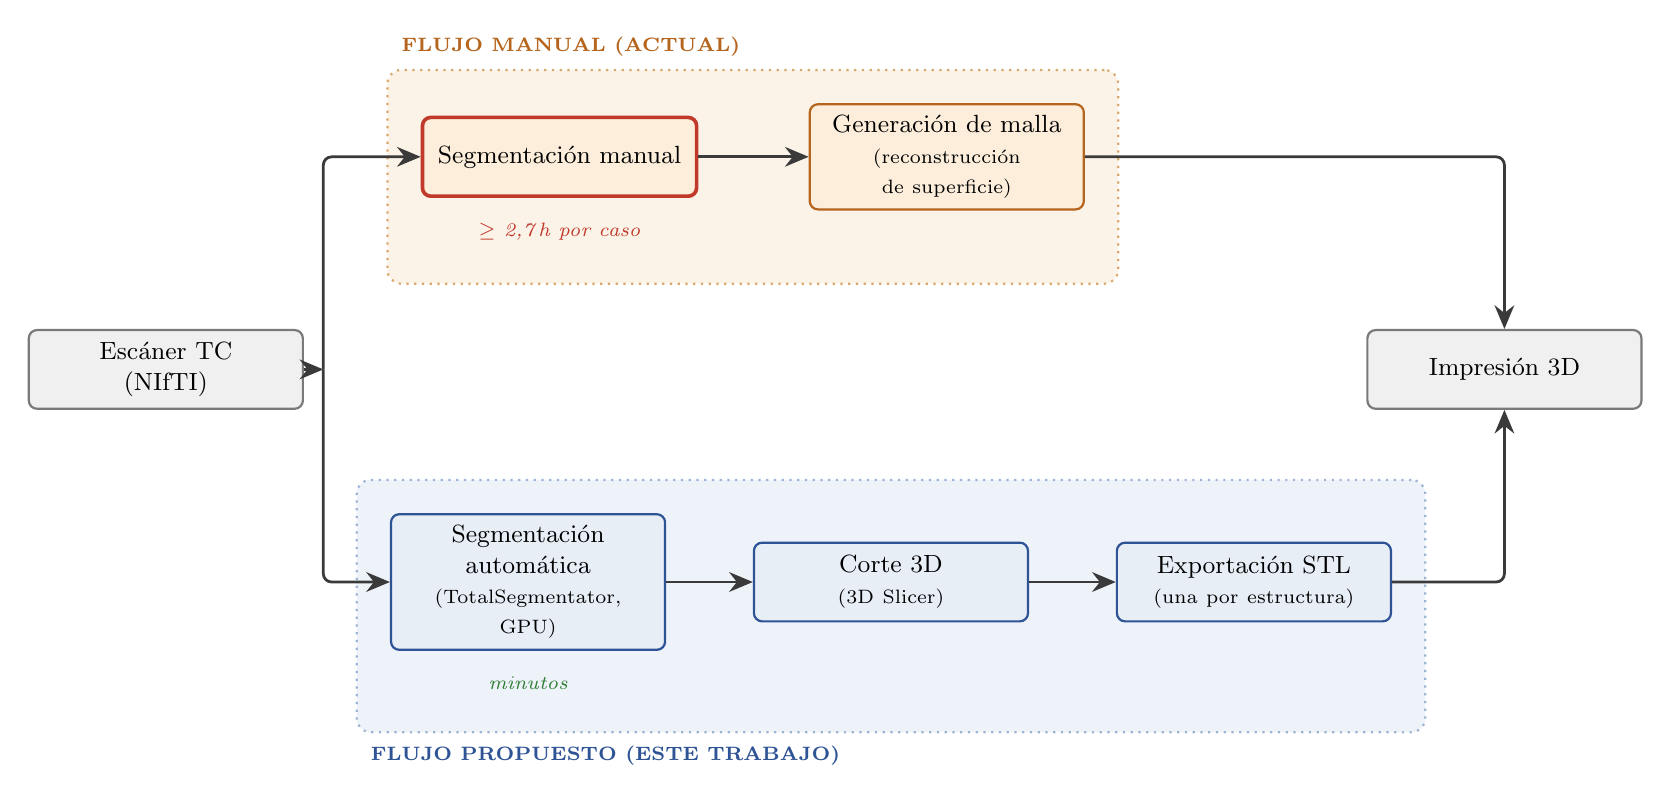
\begin{tikzpicture}[
  font=\small,
  base/.style={line width=0.8pt, rounded corners=3pt, align=center,
               text width=3.2cm, minimum height=1.0cm, inner sep=4pt},
  autobox/.style={base, draw=autoDraw, fill=autoFill},
  manualbox/.style={base, draw=manualDraw, fill=manualFill},
  botbox/.style={base, draw=botDraw, line width=1.3pt, fill=manualFill},
  sharedbox/.style={base, draw=sharedDraw, fill=sharedFill},
  flow/.style={-{Stealth[length=3mm,width=2.5mm]}, line width=1.0pt, draw=arrowCol,
               rounded corners=3pt},
  lbl/.style={font=\scriptsize\itshape, fill=white, inner sep=1.5pt},
]

% ---- Entrada compartida ----
\node[sharedbox] (tc) at (0,0) {Escáner TC\\(NIfTI)};
\coordinate (split) at (2.0,0);

% ---- Carril superior: FLUJO MANUAL ----
\node[botbox]                     (mseg)  at (5.0, 2.7) {Segmentación manual};
\node[manualbox, right=1.4cm of mseg] (mmesh) {Generación de malla\\\scriptsize(reconstrucción de superficie)};

% ---- Carril inferior: FLUJO PROPUESTO ----
\node[autobox]                    (aseg)  at (4.6,-2.7) {Segmentación automática\\\scriptsize(TotalSegmentator, GPU)};
\node[autobox, right=1.1cm of aseg]   (acorte) {Corte 3D\\\scriptsize(3D Slicer)};
\node[autobox, right=1.1cm of acorte] (astl)   {Exportación STL\\\scriptsize(una por estructura)};

% ---- Salida compartida ----
\node[sharedbox] (print) at (17.0,0) {Impresión 3D};

% ---- Flechas: bifurcación desde la entrada ----
\draw[flow] (tc.east) -- (split);
\draw[flow] (split) |- (mseg.west);
\draw[flow] (split) |- (aseg.west);

% ---- Flechas internas de cada carril ----
\draw[flow] (mseg)  -- (mmesh);
\draw[flow] (aseg)  -- (acorte);
\draw[flow] (acorte)-- (astl);

% ---- Convergencia a la salida ----
\draw[flow] (mmesh.east) -| (print.north);
\draw[flow] (astl.east)  -| (print.south);

% ---- Anotaciones de tiempo (el borde rojo de la caja marca el cuello de botella) ----
\node[font=\scriptsize\itshape, text=botDraw,  below=0.2cm of mseg] (mtime) {$\geq$ 2{,}7\,h por caso};
\node[font=\scriptsize\itshape, text=fastDraw, below=0.2cm of aseg] (atime) {minutos};

% ---- Fondos de carril ----
\begin{scope}[on background layer]
  \node[draw=laneManualDraw, line width=0.8pt, dotted, rounded corners=5pt,
        fill=laneManual, fit=(mseg)(mmesh)(mtime), inner sep=12pt] (zoneM) {};
  \node[draw=laneAutoDraw, line width=0.8pt, dotted, rounded corners=5pt,
        fill=laneAuto, fit=(aseg)(acorte)(astl)(atime), inner sep=12pt] (zoneA) {};
\end{scope}
\node[font=\scriptsize\bfseries, text=manualDraw, anchor=south west]
      at ([xshift=2pt,yshift=1pt]zoneM.north west) {FLUJO MANUAL (ACTUAL)};
\node[font=\scriptsize\bfseries, text=autoDraw, anchor=north west]
      at ([xshift=2pt,yshift=-1pt]zoneA.south west) {FLUJO PROPUESTO (ESTE TRABAJO)};

\end{tikzpicture}
\end{document}